\documentclass[
book,
%a4paper,					% alle weiteren Papierformat einstellbar
%landscape,					% Querformat
11pt,						% Schriftgr�ߟe (12pt, 11pt (Standard))
BCOR0.8cm,					% Bindekorrektur, bspw. 1 cm
%DIVcalc,					% f�hrt die Satzspiegelberechnung neu aus
twoside,					% einseitiges Layout
%twocolumn,					% zweispaltiger Satz
%openany,					% Kapitel k�nnen auch auf linken Seiten beginnen
%halfparskip*,				% Absatzformatierung s. scrguide 3.1
%notitlepage,				% in-page-Titel, keine eigene Titelseite
%chapterprefix,				% vor Kapitel�berschrift wird "Kapitel Nummer" gesetzt
%appendixprefix,			% Anhang wird "Anhang" vor die ܜberschrift gesetzt 
%normalheadings,			% ܜberschriften etwas kleiner (smallheadings)
%idxtotoc,					% Index im Inhaltsverzeichnis
%liststotoc,				% Abb.- und Tab.verzeichnis im Inhalt
%bibtotoc,					% Literaturverzeichnis im Inhalt
bibliography=totoc,
%leqno,						% Nummerierung von Gleichungen links
%fleqn,						% Ausgabe von Gleichungen linksb�ndig
%draft						% �berlangen Zeilen in Ausgabe gekennzeichnet
]{scrreprt}

% ============================ Packages ============================ 

%\usepackage[inner=3.0cm,outer=2.5cm,top=1.5cm,bottom=1.5cm,includeheadfoot]{geometry}
									% Einstellungen der Seitenr�nder
\usepackage[includeheadfoot]{geometry}
\usepackage[T1]{fontenc}				% neue Rechtschreibung
\usepackage[latin1]{inputenc}		         % Umlaute erm�glichen
\usepackage[german, english]{babel}
\usepackage{fancyhdr}				% f�r Kopf- und Fuߟzeile
\usepackage[hyperref]{xcolor}		
\definecolor{MyBlue}{RGB}{50,79,132}		% f�r Kopf- und Fu�zeile
\usepackage[colorlinks, citecolor=MyBlue, linktocpage, linkcolor=MyBlue]{hyperref}
\usepackage{color}					% Farbe
\usepackage[pdftex]{graphicx}
\usepackage{float}
\usepackage{listings}				% Programm-Code
\usepackage{longtable}				% Tabellen �ber mehrere Seiten
\usepackage{siunitx}				% Einheiten nach SI-Norm
\usepackage{listings}                                    % Verwendung von Matlab-Code
\usepackage{amsmath}
\usepackage{amssymb}
\usepackage{mathtools}
\usepackage[tight]{subfigure}
\usepackage{empheq}
\usepackage{overcite}
\usepackage{url}
\usepackage{framed}
\usepackage{pdfpages}
\usepackage[compact]{titlesec}
% ============================ Kopf- und Fu�zeile ==========================

\pagestyle{fancy}
\fancyhf{}

\fancyhead[CO,CE]{\scshape\leftmark}	% Kopfzeile links [L], mitte [C], rechts [R]
\fancyfoot[RO,LE]{\thepage}				% Fu�zeile
\renewcommand{\headrulewidth}{0.5pt}	% Linie oben
\renewcommand{\footrulewidth}{0pt}		% Linie unten
\pagenumbering{roman}

%============================ new Definitions ============================
%============================ Befehlsdefinitionen============================

\newcommand{\beq}{\begin{eqnarray}}		% Abk�rzung f�r nummerierte Gleichungen
\newcommand{\eeq}{\end{eqnarray}}		% Ab�rzung f�r nummerierte Gleichungen
\newcommand{\nn}{\nonumber}				% Abk�rzung f�r nummernlose Gleichung
\newcommand{\dm}{\mathrm{d}}			% Abk�rzung f�r Differential/Integral d
\newcommand{\del}{\partial}				% Partielle Ableitung
\newcommand{\bal}{\begin{aligned}}
\newcommand{\eal}{\end{aligned}}
\newcommand*\widefbox[1]{\fbox{\hspace{2em}#1\hspace{2em}}}
\renewcommand\citeform[1]{[#1]}


\setcounter{secnumdepth}{3}
%\setlength{\subfigtopskip}{cm}
% ==================  New Chapter/Section Definition  =====================

%\titleformat{?command?}[?shape?]{?format?}{?label?}{?sep?}{?before-code?}[?after-code?]
\titlespacing{\chapter}{0pt}{0pt}{20pt}
\titleformat{\chapter}[display]{\bfseries\Large \color{MyBlue}}{\filleft \fontsize{50}{20} \selectfont \thechapter}{.5em}{\titlerule \vspace{2ex}}[\vspace{2ex} \titlerule]
\titleformat{\section}
  {\normalfont \filcenter \large\bfseries \color{MyBlue}}{\thesection}{1em}{}
%========================= Document ==============================
\newcommand{\LMUTitle}[9]{
  \thispagestyle{empty}
  \vspace*{\stretch{1}}
  {\parindent0cm
   \rule{\linewidth}{.7ex}}
  \begin{flushright}

    \vspace*{\stretch{1}}
    \sffamily\bfseries\Huge
    #1\\
    \vspace*{\stretch{1}}
    \sffamily\bfseries\large
    #2
    \vspace*{\stretch{1}}
  \end{flushright}
  \rule{\linewidth}{.7ex}
  \vspace*{\stretch{5}}
  \begin{center}
    
\includegraphics[width=2in]{Pictures/siegel}
  \end{center}
  \vspace*{\stretch{1}}
  \begin{center}\sffamily\LARGE{#5}\end{center}
  \newpage
  \thispagestyle{empty}

  \cleardoublepage
  \thispagestyle{empty}

  \vspace*{\stretch{1}}
  {\parindent0cm
  \rule{\linewidth}{.7ex}}
  \begin{flushright}
    \vspace*{\stretch{1}}
    \sffamily\bfseries\Huge
    #1\\
    \vspace*{\stretch{1}}
    \sffamily\bfseries\large
    #2
    \vspace*{\stretch{1}}
  \end{flushright}
  \rule{\linewidth}{.7ex}

  \vspace*{\stretch{3}}
  \begin{center}
    \Large Masterarbeit\\
    \Large am Lehrstuhl #4\\
    \Large der Ludwig--Maximilians--Universit�t\\
    \Large M�nchen\\
    \vspace*{\stretch{1}}
    \Large vorgelegt von\\
    \Large #2\\
    \Large aus #3\\
    \vspace*{\stretch{2}}
    \Large M�nchen, den #6
  \end{center}

  \newpage
  \thispagestyle{empty}

  \vspace*{\stretch{1}}

  \begin{flushleft}
    \large Erstgutachter:  #7 \\[1mm]
    \large Zweitgutachter: #8 \\[1mm]
  \end{flushleft}

  \cleardoublepage
}
% =============================Titelseite ==================================

\begin{document}

\pagenumbering{roman}

  \LMUTitle
      {Dies ist Titel der Masterarbeit \\
       This is the title of the thesis}               % Titel der Arbeit
      {David Symhoven}                       % Vor- und Nachname des Autors
      {Witten}                             % Geburtsort des Autors
      {Computational \& Plasma Physics}                         % Name des Lehrstuhls
      {M�nchen 2017}                          % Ort und Jahr der Erstellung
      {30.06.2017}                            % Tag der Abgabe
      {Prof.Dr.Hartmut Ruhl}                          % Name des Erstgutachters
      {Zweitgutachter}                         % Name des Zweitgutachters


%================================= ABSTRACT==============================
\begin{abstract}
\begin{center}
\textbf{Abstract:}\\
Blah Blah Blah Mr. Freeman
\end{center} 
\end{abstract}

%================================= SYMBOLE UND KONTANTEN ================
%\chapter*{Symbols and Constants}


\begin{tabular}{lll}
%Plank'sches Wirkungsquantum  	& \qquad h  			&  \qquad 6.62606957(29) $\cdot 10^{-34}~\si{\joule\second}$ \\ 
%Plank'sches Wirkungsquantum	  	&  \qquad $\hbar$  		&  \qquad1.054571726(47) $\cdot 10^{-34}~\si{\joule\second}$ \\
%Boltzmann - Konstante			& \qquad $k_{B}$ 		& \qquad  1.3806488(13) $\cdot 10^{-23}~\si{\joule\per\kelvin}$\\
%Avogadro - Konstante			& \qquad $N_A$ 		& \qquad 6.02214129(27) $\cdot 10 ^{23}~\si{\per\mole}$\\
Vacuum permittivity				& \qquad $\epsilon_0$	& \qquad 8.85418781762 $\cdot 10 ^{-12}~\si{\ampere\second\per\volt\per\meter}$\\
Vacuum permeability				& \qquad $\mu_0$		& \qquad 2566370614 $\cdot 10 ^{-6}~\si{\newton\per\square\ampere}$\\
%atomare Masseneinheit			& \qquad u 			& \qquad 1.660538921(73) $\cdot 10^{-27} ~\si{\kilogram}$\\
%Elektronenvolt					& \qquad eV			& \qquad 1.602176565(35) $\cdot 10^{-19}~\si{\joule}$\\
\noalign{\vskip 5mm}
Electrical flux density				& \qquad $\vec{D}$		& \qquad $[\si{\ampere\second\per\square\meter}]$\\
Magnetic flux density				& \qquad $\vec{B}$		& \qquad $[\si{\tesla}]$\\
Magnetic field strength			& \qquad $\vec{H}$		& \qquad $[\si{\ampere\per\meter}]$\\
Electric field stength				& \qquad $\vec{E}$		& \qquad $[\si{\volt\per\meter}]$\\
%1 Angstr�m 					& \qquad $\si{\angstrom}$  	& \qquad  $10^{-10}~\si{\meter}$ \\
%1 Nanosekunde 				& \qquad $\si{\nano\second}$  	& \qquad $10^{-9}~\si{\second}$ \\
%1 Pikosekunde 					& \qquad $\si{\pico\second}$ 	& \qquad $10^{-12}~\si{\second}$ \\
%1 Femtosekunde				& \qquad $\si{\femto\second}$ 	& \qquad $10^{-15}~\si{\second}$ \\

\noalign{\vskip 5mm}

%Ort							& \qquad $\vec{r}$			& \qquad $[\si{\meter}]$\\
%Geschwindigkeit				& \qquad $\vec{v}$ 			& \qquad $[\si{\meter\per\second}]$ \\
%Beschleunigung				& \qquad $\vec{a}$ 			& \qquad $[\si{\meter\per\square\second}]$ \\ 
%Impuls						& \qquad $\vec{p}$			& \qquad $[\si{\kilogram\meter\per\second}]$ \\
%Kraft							& \qquad $\vec{F}$ 			& \qquad $[\si{\newton}]$ \\
%Masse						& \qquad m 				& \qquad $[\si{\kilogram}]$ \\
%Energie						& \qquad E 				& \qquad $[\si{\joule}]$ \\
%Temperatur					& \qquad T				& \qquad $[\si{\kelvin}]$ \\
%Druck						& \qquad p 				& \qquad $[\si{\newton\per\square\meter}]$ \\	
%Entropie						& \qquad S				& \qquad $[\si{\joule\per\kelvin}]$ \\
%Potential						& \qquad V				& \qquad \text{nicht eindeutig} \\
%chemisches Potential			& \qquad $\mu$			& \qquad \text{nicht eindeutig} \\
%Zeit 							& \qquad t 				& \qquad $[\si{\second}]$\\
%diskretisierte Zeit				& \qquad $\Delta t$			& \qquad $[\si{\second}]$\\
%Frequenz						& \qquad $\omega$			& \qquad $[\si{\per\second}]$\\
%Gesamtteilchenanzahl			& \qquad N				& \\
%Anzahl der Freiheitsgerade		& \qquad $f$				& \\
%\noalign{\vskip 5mm}

Nabla - Operator				& \qquad $\nabla$			& \qquad  $\left( \frac{\del }{\del r_1}, \ldots, \frac{\del }{\del r_n}\right)$ \\
\noalign{\vskip 2mm}
Laplace - Operator				& \qquad $\Delta$			& \qquad  $\sum_{i=1}^{n} \frac{\del^2}{\del r_i^2}$\\
d'Alembert - Operator			& \qquad $\hat\square$		& \qquad $\Delta- \frac{1}{c^2}\frac{\del^2}{\del t^2}$\\
%\noalign{\vskip 2mm}
%Hamilton - Operator				& \qquad $\mathcal{H}$		& \qquad $\mathcal{H} = -\frac{\hbar^2}{2m}\Delta + V(\vec{r})$ \\		
%\noalign{\vskip 2mm}
%Lagrange - Funktion				& \qquad $\mathcal{L}$		& \qquad $\mathcal{L} = T - V$ \\

\end{tabular}


%================================= Inhaltsverzeichnis ==========================
\tableofcontents

%============================ Beginn Textseiten ================================
\pagenumbering{arabic}



%================================= Bildvorlage ====================================

%Code f�r Bildumgebung
%\begin{figure}[H]
%	\centering
%		\includegraphics[width=0.50\textwidth]{Destruktive_Interferenz.jpg} %Bild 1
%	\caption[Destruktive Interferenz]{Destruktive Interferenz \cite{[Wiki12]}}
%	\label{fig:Interferenzfilterr}
%\end{figure}
%\noindent

%===========================================================================


%======================== EINLEITUNG ========================
%===========================================================
\chapter{Introduction}
Now it's going loose ...  \cite{Allen}

\chapter{Fundamentals}
%======================== LW Potentials ========================
%===========================================================
\section{Li�nard-Wiechert Potentials}
\beq
\label{eqn: Li�nard-Wiechert}
\bal
E = E \\
B = B 
\eal
\eeq
\label{sec: lw-potentials}

%======================== Numerics ========================
%===========================================================
\section{Numerics}
\noindent
The following section deals with the numeric aspects of this thesis. We explain the underlying equation of motions and their history. After that, we go into several methods with which we can solve differential equations. Over the course of the last decades numerous methods were invented each of which has its own strength and weaknesses. 
Some of them are very easy to implement, which in turn usually leads to unprecise results. Others are quite complicated and sophisticated to implement, but very accurate.
Therefore one should always consider which method is best for the problem and what it is one want to achieve.\\
Following this, we also want to define and calculate the numerical complexity of some chosen algorithms. 

%======================== Equation of Motion ========================
\subsection{Equations of motion}
As we know from mechanics the dynamic of a particle is determined by the forces acting on it. In our case there is a force due to electro-magnetic fields. That can be external fields, but also fields due to moving particles, as we explained in section \ref{sec: lw-potentials}.\\
The dynamics of our system is described by the \textit{Lorentz-Newton} equation
\beq
\label{eqn: Lorentz-Newton}
\bal
\frac{\dm x^{\mu}}{\dm \tau} &= u^{\mu}\\
\frac{\dm u^{\mu}}{\dm \tau} &= F^{\mu}_{~\nu}~u^{\nu} + g^{\mu},
\eal
\eeq
which derivation is quite longish, why we want to refer to literature. \\%MISSING: cite
The term $F^{\mu}_{~\nu}$ describes the electromagnetic field strength tensor
\beq
F^{\mu}_{~\nu} = 
\begin{pmatrix}
0 & E_x & E_y & E_z \\
E_x & 0 & B_z & -B_y \\
E_y & -B_z & 0 & B_x \\
E_z & B_y & -B_x & 0
\end{pmatrix}
.
\eeq
The damping term $g^{\mu}$ considers the fact that charged particles radiate fields when they are moving which leads to a loss in their kinetic energy. Within the context of classical electrodynamics Max \textit{Abraham} and Hendrick \textit{Lorentz} discussed radiation damping in their same-named equation first.
In 1938 \textit{Dirac} generalized the equation whilst taking special relativity into account. \\% MISSING: Cites
% MISSING: Details. Historisches. Abraham, Lorentz, Dirac Landau Lifschitz Gleichung usw.
We now want to deal with how to solve the Lorentz-Newton equation \eqref{eqn: Lorentz-Newton} numerically.

%======================== Euler Scheme ========================
\subsection{Euler-Scheme}
The most simple method is the explicit \textit{Euler}-Method. It's easy to implement but not very accurate, as we shall see later. But before we go into the details of the explicit Euler-Scheme we need to address some prerequisites all following methods will have in common. \\
Starting point will always be a first order system of the kind
\beq
\label{eqn: Euler}
\bal
\frac{\dm x^{\mu}}{\dm \tau} &= u^{\mu}\\
\frac{\dm u^{\mu}}{\dm \tau} &= f^{\mu}(x^{\nu},u^{\nu})\\
x^{\mu}(\tau_0) &= x^{\mu}_0\\
u^{\mu}(\tau_0) &= u^{\mu}_0.
\eal
\eeq
Systems of higher order can always be reduced to a first order system. \\
In order to solve the equation of motion numerically the domain needs to be discretized. Therefore we divide the time interval into N equidistant partial intervals $h$, by defining
\beq
h \coloneqq \Delta \tau = \tau_{i+1} - \tau_i. \nn
\eeq
The idea is to calculate each point along the trajectory $x^{\mu}_i = x^{\mu}(\tau_i)$ iteratively, starting from the initial values $x^{\mu}_0$ and $u^{\mu}_0$.
But to calculate these points all differential operators in  \eqref{eqn: Euler} need to be discretized as well. That is where all methods differ. Each method has its own way to discretize the differential operators.\\
The basis of the Euler-Scheme is a first order Taylor expansion of the integration variable $x^{\mu}$ in $\tau$ around $\tau_i$
\beq
\label{eqn: Taylor}
x^{\mu}(\tau_{i+1}) =  x^{\mu}(\tau_i) + \frac{\dm x^{\mu}}{\dm \tau} \Big |_{\tau=\tau_i} \underbrace{(\tau_{i+1} - \tau_i)}_{=h} + \mathcal{O}(h^2).
\eeq
Analogously for $u^{\mu}$ and solving for  $\frac{\dm x^{\mu}}{\dm \tau}$ and $\frac{\dm u^{\mu}}{\dm \tau}$ respectively yields
\beq
\bal
\frac{x^{\mu}_{i+1} - x^{\mu}_i}{h} &= u^{\mu}_i\\
\frac{u^{\mu}_{i+1} - u^{\mu}_i}{h} &= f^{\mu}(x^{\nu}_i,u^{\nu}_i).
\eal
\eeq
This way of discretizing allows a very easy calculation of $x^{\mu}_i$ according to
 \beq
\bal
x^{\mu}_{i+1} &= x^{\mu}_i + h~u^{\mu}_i\\
u^{\mu}_{i+1} &= u^{\mu}_i + h~f^{\mu}(x^{\nu}_i,u^{\nu}_i).
\eal
\eeq
In order for us to calculate the goodness of this approximation we need to introduce the \textit{Procedural Error} and the \textit{Order of Consistency} \cite{NumerikSkript}.\\
\subsubsection{Procedural Error  and Order of Consistency}
\newtheorem{env_definition}{Definition}[section]
\begin{env_definition}[Procedural Error  and Order of Consistency]
\label{def: Procedural Error}
Let $I \subseteq \mathbb{R}$ be a interval, $f : I \times \mathbb{R}^d \to \mathbb{R}^d$, $y : I \to \mathbb{R}^{d}$ a solution of the initial value problem
\beq
\bal
\frac{\dm}{\dm \tau}y(\tau) &= f(\tau,y(\tau)),\\
y(\tau_0) &= y_0. 
\eal
\eeq
\begin{description}
\item[(a)] The term 
\beq
\eta(\tau,h) \coloneqq y(\tau) + h f(\tau, y(\tau)) - y(\tau+h)\quad \text{for}~\tau \in I,~ 0 < h \le b - \tau
\eeq
is called local Procedural Error of the One-Step-Scheme at $\tau$ for the increment h.
\item[(b)] The One-Step-Scheme has an Order of Consistency $p \ge 1$, if the local Procedural Error fulfils
\beq
||\eta(\tau,h) || \le Ch^{p+1}\quad \text{for}~\tau \in I,~ 0 < h \le b - \tau,
\eeq 
with a constant $C\ge 0$, which is independent of $\tau$ and $h$.
\end{description}
\end{env_definition}
Descriptively the Procedural Error is the difference between the exact solution $y(\tau+h)$ and the result, which we get from the One-Step-Scheme starting from the exact solution at the earlier time step $y(\tau)$.
Figure \ref{fig: Procedural Error} illustrates the situation.
\begin{figure}[H]
	\centering
		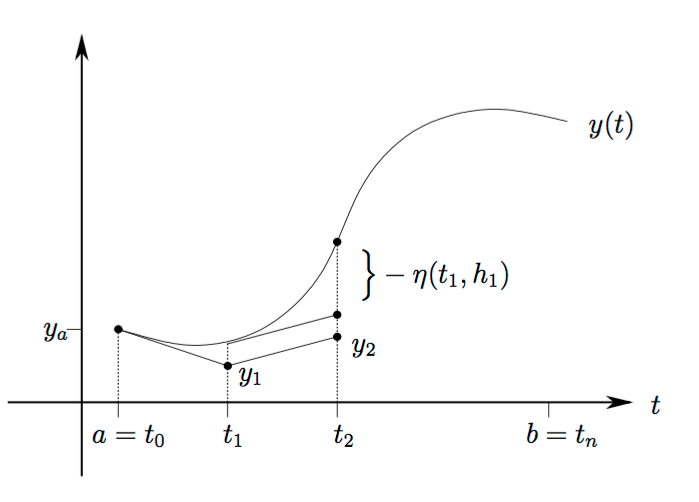
\includegraphics[width=0.50\textwidth]{Pictures/Verfahrensfehler.png} %Bild 1
	\caption[Procedural Error]{Illustration of the Procedural Errors of an One-Step-Scheme.~ \cite{NumerikSkript}}
	\label{fig: Procedural Error}
\end{figure}
\noindent
We now want to use the definitions \ref{def: Procedural Error} to calculate the Order of Consistency of the Euler-Scheme.\\
Starting point is the system \eqref{eqn: Lorentz-Newton}. Thereby we focus on the equation for $u^{\mu}$, since $x^{\mu}$ can be easily integrated from $u^{\mu}$.
Following Definition \ref{def: Procedural Error} we have
\beq
y = u^{\mu}. \nn \\
\eeq
We get
\beq
\label{eqn: eta u}
\eta(\tau, h) = u^{\mu}(\tau_i) + h f^{\mu}(x^{\nu}, u^{\nu}) - u^{\mu}(\tau_{i+1}).
\eeq
The last term can be calculated with a Taylor-expansion analogously to \eqref{eqn: Taylor}.
\beq
\label{eqn: Taylor u}
u^{\mu}(\tau_{i+1}) =  u^{\mu}(\tau_i) + h~\frac{\dm u^{\mu}}{\dm \tau} \Big |_{s=\tau_i}  + h^2~\frac{\dm^2 u^{\mu}}{\dm \tau^2} \Big |_{s=\tau_i}.
\eeq
Plugging in \eqref{eqn: Taylor u} in \eqref{eqn: eta u} yields
\beq
\bal
\eta(\tau, h) &= u^{\mu}(\tau_i) + h\frac{\dm u^{\mu}}{\dm \tau}  - u^{\mu}(\tau_{i+1}) \\
\stackrel{ \eqref{eqn: Taylor u}}{\Longrightarrow}\eta(\tau, h) &= u^{\mu}(\tau_i) + h\frac{\dm u^{\mu}}{\dm \tau}  - u^{\mu}(\tau_i) - h\frac{\dm u^{\mu}}{\dm \tau} - h^2\frac{\dm^2 u^{\mu}}{\dm \tau^2}\\
\Longleftrightarrow\eta(\tau, h) &= \frac{\dm^2 u^{\mu}}{\dm \tau^2}~h^2 ,
\eal
\eeq
since $\frac{\dm u^{\mu}}{\dm \tau} = f^{\mu}(x^{\nu}, u^{\nu})$ holds for the Euler-Scheme. Thus
\beq
|\eta(\tau, h)| \le C h^2 \quad \text{with}~C \coloneqq \frac{1}{2} \max_{\tau \in \mathcal{D}(u^{\mu})}\left| \frac{\dm^2 u^{\mu}}{\dm \tau^2}\right|.
\eeq
$\mathcal{D}(u^{\mu})$ denotes the domain of $u^{\mu}$. Therefore, the Euler-Scheme has an Order of Consistency of one.


%======================== Leap Frog Scheme ========================
\subsection{Leap-Frog-Scheme}
A definitely better method is the so called \textit{Leap-Frog}-Scheme. One can easily proof that it has an Order of Consistency of two. \\
In contrast to the explicit Euler-Scheme this method has several advantages. For one it is time reversible, i.e. it is possible to reach any previous point in time from every point later in the trajectory. On the other hand the Leap-Frog-Scheme is symplectic, meaning it conserves the phase space volume from which energy and momentum conservation follows. \\
However, one disadvantage is that it's only suited for systems in which the acting force exclusively depends on the current position, but not on the velocity of the particle. This would lead to an implicit equation system which is numerically way more expensive to solve. \\
Thus the differential equation should be of the form
\beq
\frac{\dm^2 x^{\mu}}{\dm \tau^2} = \frac{\dm u^{\mu}}{\dm \tau} = f^{\mu}(x^{\nu}).
\eeq
As we already mentioned, the various methods discretize the differential operators differently
The Leap-Frog-Scheme uses
\beq
\bal
\frac{x^{\mu}_{i+1} - x^{\mu}_i}{h} &= u^{\mu}_{i+\frac{1}{2}}\\
\frac{u^{\mu}_{i+\frac{1}{2}} - u^{\mu}_{i-\frac{1}{2}}}{h} &= f^{\mu}(x^{\nu}_i).
\eal
\eeq
Solving for the new time step yields
\beq
\bal
x^{\mu}_{i+1} &= x^{\mu}_i + h u^{\mu}_{i+\frac{1}{2}}\\
u^{\mu}_{i+\frac{1}{2}} &= u^{\mu}_{i-\frac{1}{2}} + h f^{\mu}(x^{\nu}_i).
\eal
\eeq
\noindent
As we can see, position and velocity are calculated at different times. They are shifted against each other in time by $h = \frac{1}{2}$. \\
But what if we have a system in which the force depends on the velocity ? Are we stuck with expensive implicit methods ? Fortunately not. We can use the \textit{Boris} - Method.
\subsection{Boris-Method}
This method was invented in 1970 by J.P. Boris \cite{boris} and is the standard method for pushing particles in plasma simulations today. We want to solve the Lorentz-Newton equation
\beq
\label{eqn: LorentzNewton}
\bal
\frac{v_{i+\frac{1}{2}} - v_{i - \frac{1}{2}}}{h} &= \frac{q}{m}\left(\vec{E} + \frac{v_{i+\frac{1}{2}} + v_{i - \frac{1}{2}}}{2} \times \vec{B}\right)
\eal
\eeq
Boris noticed, that upon defining
\beq
\label{eqn:vMinusAndPlus}
\bal
\vec{v}_{-} &\coloneqq v_{i - \frac{1}{2}} + \frac{h}{2}\frac{q \vec{E}}{m}\quad\text{and} \\
\vec{v}_{+} &\coloneqq v_{i + \frac{1}{2}} + \frac{h}{2}\frac{q \vec{E}}{m},
\eal
\eeq
one can eliminate the electric field. Plugging in \eqref{eqn:vMinusAndPlus} into \eqref{eqn: LorentzNewton} yields
\beq
\bal
\frac{\vec{v}_{+} - \vec{v}_{-}}{h} = \frac{q}{m} (\vec{v}_{+} + \vec{v}_{-}) \times \vec{B}.
\eal
\eeq
Following the geometrical analysis in ~\cite{Birdsall} we find %MISSING:PIctures from Birdsall and rest of explaination
\begin{figure}[H]
	\centering
		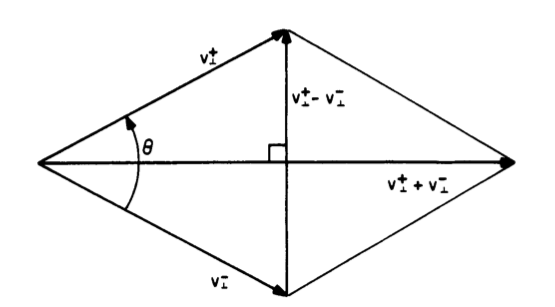
\includegraphics[width=0.70\textwidth]{Pictures/borisRotation.png} 
	\caption[Caption]{Blah Blah}
	\label{fig: borisRotation}
\end{figure}
\noindent

\begin{figure}[H]
	\centering
		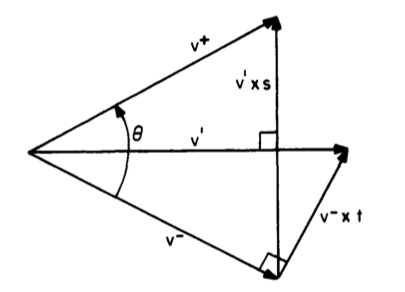
\includegraphics[width=0.70\textwidth]{Pictures/borisProjection.png} 
	\caption[Caption ]{Blah Blah}
	\label{fig: borisProjection}
\end{figure}
\noindent

%======================== Interpolation of Trajectories ========================
\subsection{Interpolation of Trajectories}
\label{sec: Interpolation of Trajectories}
The previously presented methods calculate the particle trajectory solely at discrete points in time $x_i^{\mu}(\tau)$. Calculating Li�nard-Wiechert fields according to equation \eqref{eqn: Li�nard-Wiechert} however, requires the intersection point of the trajectory with the backward lightcone of the observation point. 
In most cases the calculated points of the trajectory are not lying directly on the lightcone, so we need a procedure to calculate the intersection point exactly.\\
The simplest solution is a linear interpolation between the last point inside and the first point outside the lightcone. Figure \ref{fig: Interpolation} illustrates the situation.
\begin{figure}[H]
	\centering
		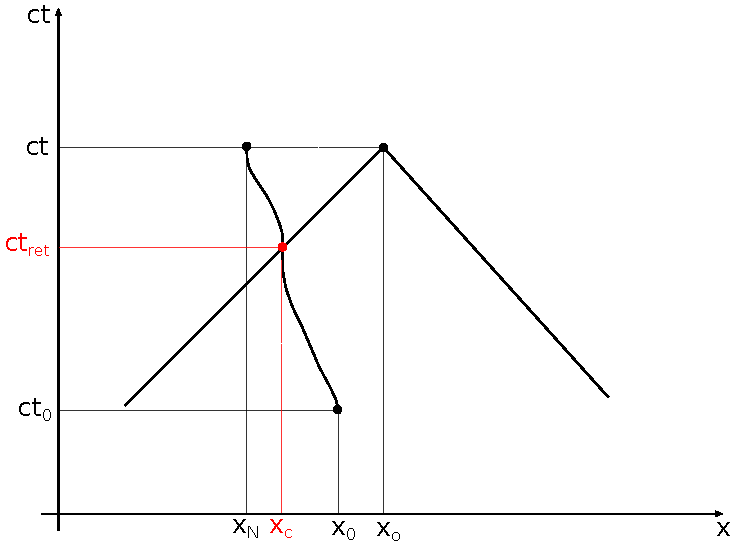
\includegraphics[width=0.80\textwidth]{Pictures/LightconeNew.pdf}
	\caption[Interpolation of Trajectories]{Minkowski space showing the particle trajectory with starting point $x^{\mu}_0(t_0)$ and last point $x^{\mu}_N(t)$. The observation point $x^{\mu}_o(t)$ with its backward lightcone is also shown. If we want to calculate the Li�nard-Wiechert fields at the observation point $x^{\mu}_o(t)$, we need the intersection point $x^{\mu}_c(t_{ret})$ of the trajectory with the backward lightcone. }
	\label{fig: Interpolation}
\end{figure}
\noindent
Thereto let $x_j^{\mu} \in \mathbb{R}^{3+1}$ be the last point inside and $x_{j+1}^{\mu} \in \mathbb{R}^{3+1}$ the first point outside the lightcone. Further let $x_{c}^{\mu} \in \mathbb{R}^{3+1}$ be the intersection point of interest then we get
\beq
\label{eqn: linInt}
x_c^{\mu} = x_j^{\mu} + \lambda ~\left(x_{j+1}^{\mu} - x_j^{\mu}\right),
\eeq
where $\lambda \in [0,1]$. Due to the finite speed of light the intersection point $x_c^{\mu}$ needs to fulfill
\beq
\label{eqn: constraint}
\left| \vec{x}_o(t) - \vec{x}_c(t_{ret})\right| = c~(t - t_{ret}) \Longleftrightarrow (x_o - x_c)_{\mu} (x_o - x_c)^{\mu} = 0.
\eeq
Thereby $x_o^{\mu} \in \mathbb{R}^{3+1}$ denotes the observation point where the fields shall be calculated. Note, that on the left hand side of \eqref{eqn: constraint} only spatial components of the respective four vectors are used. \\
Plugging in \eqref{eqn: linInt} in \eqref{eqn: constraint} yields

\begin{multline}
\label{eqn: quadEq}
\lambda^2 (x_{j+1} - x_j)_{\mu}(x_{j+1} - x_j)^{\mu} + \lambda~2(x_{j+1} - x_j)_{\mu}(x_j - x_o)^{\mu} + (x_j)_{\mu}(x_j)^{\mu} \\ + (x_o)_{\mu}(x_o)^{\mu} - 2(x_j)_{\mu}(x_o)^{\mu}  = 0.
\end{multline}
We define
\beq
\bal
a &\coloneqq (x_{j+1} - x_j)_{\mu}(x_{j+1} - x_j)^{\mu}\\
b &\coloneqq 2(x_{j+1} - x_j)_{\mu}(x_j - x_o)^{\mu} \\
c &\coloneqq (x_j)_{\mu}(x_j)^{\mu} + (x_o)_{\mu}(x_o)^{\mu} - 2(x_j)_{\mu}(x_o)^{\mu}. \nn
\eal
\eeq
In general the quadratic equation \eqref{eqn: quadEq} in $\lambda$ has two solutions
\beq
\lambda_{1/2} = \frac{-b \pm \sqrt{b^2 - 4ac}}{2a}. \nn
\eeq
One denotes the intersection point with the backward lightcone, the other one with the forward lightcone. Since  $\lambda \in [0,1]$ we are only interested in the larger one. 
\beq
\lambda_{1/2} = \frac{-b + \sqrt{b^2 - 4ac}}{2a}. \nn
\eeq
Plugging in $\lambda$ in \eqref{eqn: linInt} gives the desired intersection point.

%======================== Hybrid Fields ========================
%===========================================================
\section{Hybrid Fields}
In this section we introduce the concept of hybrid fields and how this approach reduces the numerical complexity from $N^2$ to $N$.\\
Usually the numerical complexity of multi particle simulation is $N^2$, due to the interaction between each particle. In our case we need $N$ push operations for the particles. One push for each particle. In order to do that, however, we need to solve equation \eqref{eqn: Lorentz-Newton} and therefore all Li�nard-Wiechert fields from the other $N-1$ particles are needed. This results in $N(N-1)$ calculations for each time step, period. If we want to calculate the Li�nard-Wiechert fields, we also need to store all positions from all particles, as explained in section \ref{sec: Interpolation of Trajectories}. For a few particles such simulations are effortlessly feasible. But with increasing particle numbers such simulations may not just require more and more memory capacity but also become so time consuming that at some point we simply can not do them anylonger. That's where the hybrid field model comes in. Instead of calculating the Li�nard-Wiechert fields at every time step for all particles at all grid points we save them onto the grid and propagate them through the grid using Maxwell equations. How that works in detail is explained in the following sections. 
\subsection{Maxwell-Equations}
% MISSING: Which one to use ? For Maxwell Pusher  the vacuum equations are suffice. For UPML we need the ones in anisotropic media
The Maxwell equations are the foundation of the classical electromagnetism and describe how the electric field $\vec{E} \in \mathbb{R}^3$ and the magnetic field $\vec{H} \in \mathbb{R}^3$ are generated by charges and currents respectively and how they evolve over time in space in presence of one another. In homogenous and isotropic media the Maxwell Equations read
\beq
\label{eqn: maxwellEq}
\bal
\epsilon_0\epsilon_r \vec{\nabla} \vec{E} &= \rho \\
\mu_0\mu_r \vec{\nabla} \vec{B} &= 0\\
\vec{\nabla} \times \vec{E} &= - \mu_0\mu_r \frac{\del \vec{B}}{\del t}\\
\vec{\nabla} \times \vec{H} &=  \epsilon_0\epsilon_r \frac{\del \vec{E}}{\del t} + \sigma \vec{E},
\eal
\eeq
where $\epsilon_0 $ and $\epsilon_r$ are the vacuum and the relative electric permeability respectively. Same holds for $\mu_0$ and $\mu_r $ for magnetic materials.
$\rho$ denotes the current density of the electric source and $\sigma$ the electric conductivity. \\
To solve the Maxwell equations numerically we need to discretize them first. The most robust and reliable way of doing this is with the \textit{Yee-Algorithm}. 

%======================== Yee Scheme ========================
\subsection{The Yee-Scheme}
In this section we talk about how to solve the Maxwell Equations \eqref{eqn: maxwellEq} and how to propagate the fields on a numerical grid. We thereby focus on the Maxwell Equations in vacuum, i.e. $\rho = \sigma = 0$ and $\epsilon_r = \mu_r = 1$. As can be seen in the Li�nard-Wiechert formula \eqref{eqn: Li�nard-Wiechert} there is a singularity for the field values at the particle position itself. Thus, we just want to propagate fields far away from the source, which is explained in more detail later.\\
\newline 
To push the fields on the grid. i.e solving for the fields at the next time step, we use the Yee - Scheme introduced by \textit{Kane Yee} in 1966 \cite{Yee66}.\\
Figure \ref{fig: YeeBox} illustrates a so called Yee-Box and the components we need to solve the curl equations of \eqref{eqn: maxwellEq}. 
\begin{figure}[H]
	\centering
		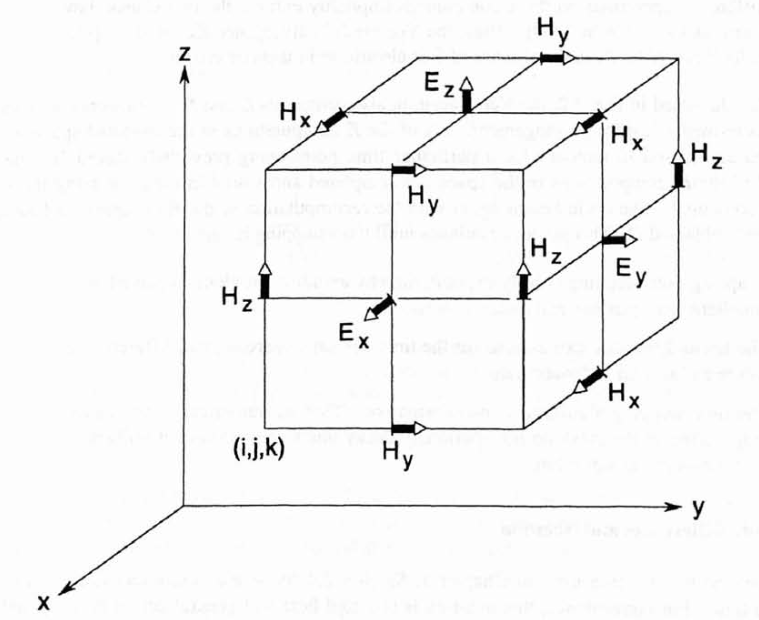
\includegraphics[width=0.70\textwidth]{Pictures/YeeBox.png} 
	\caption[Yee-Box]{An illustration of a Yee-Box which is used to solve the curl Maxwell Equations. Shown are the positions of the electric and magnetic field vector components about a cubic unit cell of the Yee space lattice.The Yee algorithm centers its E and H components in three- dimensional space so that every E component is surrounded by four circulating H components, and every H component is surrounded by four circulating E components.\cite{Taflove}.}
	\label{fig: YeeBox}
\end{figure}


%======================== Near and Far- Fields ========================
\subsection{Near-and Farfields}


%======================== UPML ============================
%===========================================================
\section{Uniaxial Perfectly Matched Layer}


%============================= Abbildungsverzeichnis ===========================
\listoffigures

%======================== Literaturverzeichnis ========================

\bibliography{reference}{}
\bibliographystyle{plain}

%================================= ERKL�RUNG=============================
\chapter*{Declaration}
\addcontentsline{toc}{chapter}{Declaration}
\vspace{1cm}
\noindent
Erkl�rung:\\
\newline
Hiermit erkl�re ich, die vorliegende Arbeit selbst�ndig verfasst zu haben und keine anderen als die in der Arbeit angegebenen Quellen und Hilfsmittel benutzt zu haben.\\
\newline
M�nchen, 17.07.2017 \\
\vspace{2cm}
\\
\line(1,0){300}\\
David Symhoven



\end{document}











